
\section {Introduction}
\subsection{Working Flow}
\begin{frame}
\frametitle{Introduction}
\footnotesize
\begin {itemize}
\item Physical interconnect network is a bottleneck when mapping applications for Multi-FPGA Network-of-Chips
\item Applications for Multi-FPGA system needs isolation from the communication network
\item NoC partitioning and implementation using multiple FPGAs will help designing larger systems
\item Challenge is the automation of NoC partitioning
\item Interconnect between FPGA has to be high speed and physically realizable
\item Implementation of DUT PG-LDPC (7,3) over partitioned and un-partitioned CONNECT generated 4 $\times$ 4 Mesh NoC
\item Utilizing Raspberry Pi with DE0-Nano for hardware-software co-design 
\end {itemize}
\normalsize
\end{frame}  

\subsection{Why is NoC used and why do we need its partitioning?}
\begin{frame}
\frametitle{Need of NoC}
\footnotesize
\begin{itemize}
\item Isolation of processing nodes and communication network
\item NoC utilizes the computer networking fundamentals and provides a communication infrastructure for designing System-on-Chip (SoC)
\item Trade-off between 
	\begin {enumerate}  
	\item Point to point transmission  \tab{- high speed and complex}
	\item Shared bus data transmission \tab{- Low speed and simpler} 
	\end {enumerate}
\item Ease of verification and logic error determination
\item By connecting computing nodes to PE of NoC, routing congestion is taken care by NoC
\item Useful to design flexible and scalable architecture implementation
\end{itemize} 
\normalsize
\end{frame}

\begin{frame}
\frametitle{Need of NoC Partitioning}
\footnotesize
\begin{itemize}
\item With the increase in number of processing cores, on-chip block RAMs, specialized IP cores etc.., packing all these onto single die using traditional interconnection techniques will no longer be feasible
\item For multi FPGA network-of-chips interconnect is the bottleneck
\item Partitioning utilizes networking fundamental and isolates the application layers and physical link layer by introducing partitioning cuts at data link layer
\item Now all the modifications and partitioning take place in data link layer making the application design and mapping independent of data exchange methods
\end{itemize} 
\normalsize
\end{frame}


% \begin{frame}
% \frametitle{Need of NoC Partitioning}
% \footnotesize
% \begin{itemize}
% \item Independence of application nodes from the communication network presents as a viable alternative
% \item Total interconnection between FPGAs reduces introducing physical interconnect delays and latency
% \item High speed serial interconnect IP cores using Gigabyte transceiver pairs can be used as inter-chip communication and data exchange unit
% \item Partial serialization / de-serialization units between FPGAs can help improving the bandwidth
% \end{itemize} 
% \normalsize
% \end{frame}
\subsection{NoC Architecture}

\begin{frame}
  \frametitle {NoC Building Blocks}
   
 \newtheorem*{link}{Links}
 \newtheorem*{router}{Router}
 \newtheorem*{network_interface}{Network Adapter (NA) or Network Interface (NI)}
    
    \begin {itemize}
      \item \begin{link}
	      The elements which physically connect the nodes and actually
	      implement the communication are called as \textit{Links}.
	    \end{link}
      
      \item \begin {router}
	      The decentralized logic which implements the communication
	      protocol is called \textit{Router}.
	    \end {router}
	    	
	
      \item \begin{network_interface}
	      The block which makes the logic connection between IP cores and network is called as 
	      Network Interface or Network Adapter.
	    \end{network_interface}
    \end {itemize}

\end{frame}


\begin {frame}
    %\newtheorem*{flit}{Flit}
     \frametitle {Router and Flit}
      \textbf{\textit{Routers}}
	\begin {itemize}
	  \item The critical part of NoC.
	  \item Receives the data packet from the adjacent router or from the attached Processing Element.
	  \item Redirects packet to the Processing Element or the next adjacent router.
	\end {itemize}

	
%    \begin{flit}
     \textbf{\textit{Flit}}
     \begin {itemize}
	  \item The physical unit, which is the minimum amount of data that is transmitted in one link transaction.  
	  \item Atomic unit that forms \textit{packets} and \textit{streams}.
      \end {itemize}
\end {frame}

\begin{frame}
    \textbf{\textit{Flow Control:}} Characterizes the packet movement across NoC channel.
      \begin {itemize}
	  \item \textit {Centralized Control:} Routing decisions made globally and applied to all nodes.
	  \item \textit {Distributed Control:} Each router makes decision locally. 
      \end {itemize}
    
    \textbf{\textit{Routing Algorithm:}} Logic that selects one output port to forward a packet 
		  that arrives at the router input.
      \begin {itemize}
	  \item \textit {Deterministic Routing:} A packet always uses the same path
				    between any set of nodes.
	  \item \textit {Adaptive Routing:} Alternate path between two nodes may be
				    used if the original path or local link is congested. 
	  \item \textit {Static Routing:} Paths between cores are defined at compilation time.
	  \item \textit {Dynamic Routing:} Paths between cores are defined during run-time.
      \end {itemize}
    
\end{frame}


\begin{frame}
    \textbf{\textit{Arbitration:}} Logic that selects one input port, 
    when multiple packets arrive at the router simultaneously requesting the same output port.
      \begin {itemize}
	  \item \textit{static} (fixed), or \textit{dynamic} (variable)
	  \item \textit{distributed} (one per port) or \textit{centralized} (one per router). 
      \end {itemize}
    
    \textbf{\textit{Buffering:}}
	  The strategy used to store information in the router during
	  congestion in the network, and the packet cannot be forwarded 
	  immediately to the correct port
    \textbf{\textit{Routing Algorithm:}} Logic that selects one output port to forward a packet 
		  that arrives at the router input.
      \begin {itemize}
	  \item \textit {Single Buffer per Router} %shared by all input ports
	  \item \textit {Single Buffer per port}
      \end {itemize}
    
\end{frame}


\begin {frame}
    \begin {itemize}
     \item \textbf {\textit{Deadlock:}} The condition when network resources are fully occupied and 
	  waiting for each other to be released for communication.
      
     \item  \textbf {\textit{Virtual Channel (VC):}} VC uses the concept of multiplexing 
	  a single physical channel over numbers of logically separate channels with 
	  individual and independent buffer queues. 

      \item The NoC used involves \textit{Distributed Flow Control} approach and \textit{Virtual Channels}.
	  NoC uses \textit{XY routing}, which is \textit{deterministic} and \textit{static} routing,
	  \textit{Round Robin} arbitration, which is \textit{distributed} and \textit{dynamic} arbitration approach, 
	  and multiple buffers (typically 8) at each input port
    \end {itemize} 
\end {frame}


%%%%%%%%% Insert diagram of NoC Topology and Routing strategy here
\begin{frame}
  \frametitle{NoC Topologies and Routing strategies}   % Insert frame title between curly braces
  \begin{columns}[c]
  \column{2in}  % slides are 3in high by 5in wide
  NoC Topologies
  \begin{itemize}
  \item Mesh 
  \item Fat-Tree
  \item Ring, Bus etc
  \end{itemize} 
  NoC Routing Strategies
  \begin{itemize}
  \item XY Routing 
 % \item Adaptive Routing
  \end{itemize}
  \column{2in}
  \includegraphics[scale=0.3]{./diagram/noc_intro_dia} 
  \end{columns}
\end{frame}


%%%%%%%%% Insert screenshot of CONNECT NoC here

\subsection{CONNECT NoC Tool}


\begin{frame}
  \frametitle{\emph{CON}figurable \emph{NE}twork \emph{C}reation \emph{T}ool \footnotemark}   % Insert frame title between curly braces
  \begin{columns}[c]
  \column{3in}  % slides are 3in high by 5in wide
  CONNECT NoC
  \begin{itemize}
  \item Developed by Michael K. Papamichael, Carnegie Mellon University 
  \item Generates fully synthesizable
  Verilog code.
  \item Latency between two adjacent Processing Element under no traffic
	is 2 cycle and +1 cycle per additional router distance.
  \item Provision of custom parameter selection\\
  i.e. Data width, number of I/O buffers, Routing strategies.\\
  \normalsize
  
  \footnotetext{\tiny{Developed by Michael Papamichael. Fast scalable FPGA-based network-on-chip simulation models.}}
  \end{itemize} 
  \column{3in}
  
  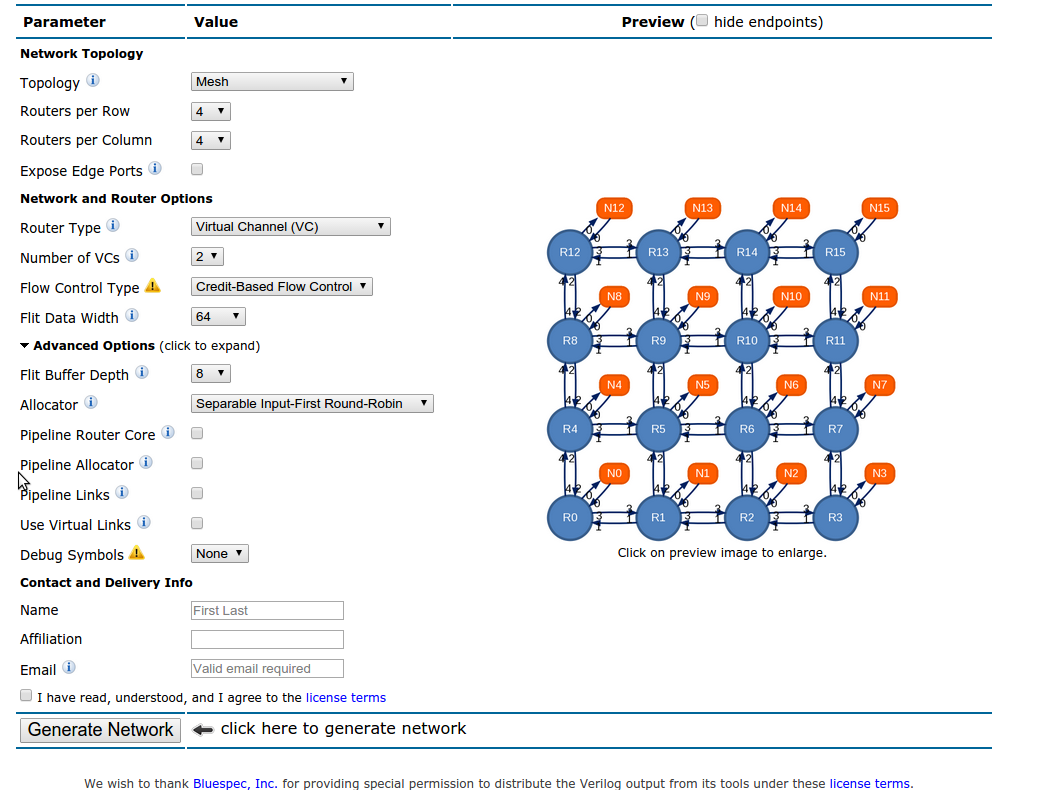
\includegraphics[scale=0.2]{./diagram/connect_noc_web}

  \end{columns}
\end{frame}




\subsection{Flit- Structure and NoC Parameters}


\begin{frame}
  \frametitle{Flit-Data structure and NoC Parameters}   % Insert frame title between curly braces
  \begin{center}

  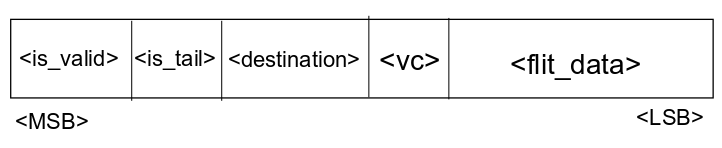
\includegraphics[scale=0.4]{./diagram/flit_structure} 
  \end{center}

\begin{table} [!h]
% \caption{NoC Parameters}
  \begin{center}
 \resizebox{0.7\textwidth}{!}
	{\begin{tabular}{||c | c||} 
 \hline
    Topology & Mesh \\ \hline
    Routers per Row & 4 \\
    Routers per Column & 4\\
    Router Type & Virtual Channel (VC) \\
    Number of VCs & 2 \\
    Flow Control Type & Credit-Based Flow Control \\
    Flit Buffer Depth & 8 \\
    Allocator & Separate-Input First Round-Robin \\
 \hline
\end{tabular}}
\end{center}

\label{noc_parameters}

\end{table}
\end {frame}


